\documentclass[]{article}
\usepackage{lmodern}
\usepackage{amssymb,amsmath}
\usepackage{ifxetex,ifluatex}
\usepackage{fixltx2e} % provides \textsubscript
\ifnum 0\ifxetex 1\fi\ifluatex 1\fi=0 % if pdftex
  \usepackage[T1]{fontenc}
  \usepackage[utf8]{inputenc}
\else % if luatex or xelatex
  \ifxetex
    \usepackage{mathspec}
  \else
    \usepackage{fontspec}
  \fi
  \defaultfontfeatures{Ligatures=TeX,Scale=MatchLowercase}
\fi
% use upquote if available, for straight quotes in verbatim environments
\IfFileExists{upquote.sty}{\usepackage{upquote}}{}
% use microtype if available
\IfFileExists{microtype.sty}{%
\usepackage[]{microtype}
\UseMicrotypeSet[protrusion]{basicmath} % disable protrusion for tt fonts
}{}
\PassOptionsToPackage{hyphens}{url} % url is loaded by hyperref
\usepackage[unicode=true]{hyperref}
\hypersetup{
            pdftitle={Untitled},
            pdfauthor={Emily G. Mantin},
            pdfborder={0 0 0},
            breaklinks=true}
\urlstyle{same}  % don't use monospace font for urls
\usepackage[margin=1in]{geometry}
\usepackage{longtable,booktabs}
% Fix footnotes in tables (requires footnote package)
\IfFileExists{footnote.sty}{\usepackage{footnote}\makesavenoteenv{long table}}{}
\usepackage{graphicx,grffile}
\makeatletter
\def\maxwidth{\ifdim\Gin@nat@width>\linewidth\linewidth\else\Gin@nat@width\fi}
\def\maxheight{\ifdim\Gin@nat@height>\textheight\textheight\else\Gin@nat@height\fi}
\makeatother
% Scale images if necessary, so that they will not overflow the page
% margins by default, and it is still possible to overwrite the defaults
% using explicit options in \includegraphics[width, height, ...]{}
\setkeys{Gin}{width=\maxwidth,height=\maxheight,keepaspectratio}
\IfFileExists{parskip.sty}{%
\usepackage{parskip}
}{% else
\setlength{\parindent}{0pt}
\setlength{\parskip}{6pt plus 2pt minus 1pt}
}
\setlength{\emergencystretch}{3em}  % prevent overfull lines
\providecommand{\tightlist}{%
  \setlength{\itemsep}{0pt}\setlength{\parskip}{0pt}}
\setcounter{secnumdepth}{0}
% Redefines (sub)paragraphs to behave more like sections
\ifx\paragraph\undefined\else
\let\oldparagraph\paragraph
\renewcommand{\paragraph}[1]{\oldparagraph{#1}\mbox{}}
\fi
\ifx\subparagraph\undefined\else
\let\oldsubparagraph\subparagraph
\renewcommand{\subparagraph}[1]{\oldsubparagraph{#1}\mbox{}}
\fi

% set default figure placement to htbp
\makeatletter
\def\fps@figure{htbp}
\makeatother

\usepackage{dcolumn} \usepackage(subfig)
\usepackage{booktabs}
\usepackage{longtable}
\usepackage{array}
\usepackage{multirow}
\usepackage{wrapfig}
\usepackage{float}
\usepackage{colortbl}
\usepackage{pdflscape}
\usepackage{tabu}
\usepackage{threeparttable}
\usepackage{threeparttablex}
\usepackage[normalem]{ulem}
\usepackage{makecell}
\usepackage{xcolor}

\title{Untitled}
\author{Emily G. Mantin}
\date{May 1, 2020}

\begin{document}
\maketitle

\subsection{R Markdown}\label{r-markdown}

This is an R Markdown document. Markdown is a simple formatting syntax
for authoring HTML, PDF, and MS Word documents. For more details on
using R Markdown see \url{http://rmarkdown.rstudio.com}.

When you click the \textbf{Knit} button a document will be generated
that includes both content as well as the output of any embedded R code
chunks within the document. You can embed an R code chunk like this:

\begin{verbatim}
## Warning: package 'pander' was built under R version 3.5.3
\end{verbatim}

\begin{longtable}[]{@{}cccccc@{}}
\caption{Analysis of Variance Model}\tabularnewline
\toprule
\begin{minipage}[b]{0.19\columnwidth}\centering\strut
~\strut
\end{minipage} & \begin{minipage}[b]{0.06\columnwidth}\centering\strut
Df\strut
\end{minipage} & \begin{minipage}[b]{0.10\columnwidth}\centering\strut
Sum Sq\strut
\end{minipage} & \begin{minipage}[b]{0.12\columnwidth}\centering\strut
Mean Sq\strut
\end{minipage} & \begin{minipage}[b]{0.12\columnwidth}\centering\strut
F value\strut
\end{minipage} & \begin{minipage}[b]{0.12\columnwidth}\centering\strut
Pr(\textgreater{}F)\strut
\end{minipage}\tabularnewline
\midrule
\endfirsthead
\toprule
\begin{minipage}[b]{0.19\columnwidth}\centering\strut
~\strut
\end{minipage} & \begin{minipage}[b]{0.06\columnwidth}\centering\strut
Df\strut
\end{minipage} & \begin{minipage}[b]{0.10\columnwidth}\centering\strut
Sum Sq\strut
\end{minipage} & \begin{minipage}[b]{0.12\columnwidth}\centering\strut
Mean Sq\strut
\end{minipage} & \begin{minipage}[b]{0.12\columnwidth}\centering\strut
F value\strut
\end{minipage} & \begin{minipage}[b]{0.12\columnwidth}\centering\strut
Pr(\textgreater{}F)\strut
\end{minipage}\tabularnewline
\midrule
\endhead
\begin{minipage}[t]{0.19\columnwidth}\centering\strut
\textbf{Treatment}\strut
\end{minipage} & \begin{minipage}[t]{0.06\columnwidth}\centering\strut
3\strut
\end{minipage} & \begin{minipage}[t]{0.10\columnwidth}\centering\strut
1486\strut
\end{minipage} & \begin{minipage}[t]{0.12\columnwidth}\centering\strut
495.3\strut
\end{minipage} & \begin{minipage}[t]{0.12\columnwidth}\centering\strut
3.371\strut
\end{minipage} & \begin{minipage}[t]{0.12\columnwidth}\centering\strut
0.05467\strut
\end{minipage}\tabularnewline
\begin{minipage}[t]{0.19\columnwidth}\centering\strut
\textbf{Residuals}\strut
\end{minipage} & \begin{minipage}[t]{0.06\columnwidth}\centering\strut
12\strut
\end{minipage} & \begin{minipage}[t]{0.10\columnwidth}\centering\strut
1763\strut
\end{minipage} & \begin{minipage}[t]{0.12\columnwidth}\centering\strut
146.9\strut
\end{minipage} & \begin{minipage}[t]{0.12\columnwidth}\centering\strut
NA\strut
\end{minipage} & \begin{minipage}[t]{0.12\columnwidth}\centering\strut
NA\strut
\end{minipage}\tabularnewline
\bottomrule
\end{longtable}

\begin{table}[!h]

\caption{\label{tab:unnamed-chunk-1}Mean values of nitrogen and phosphorus content measured in the fall of the establishment year (2019).}
\centering
\begin{tabu} to \linewidth {>{\raggedright\arraybackslash}p{8cm}>{\raggedleft}X>{\raggedleft}X}
\toprule
Treatment & Nitrogen Content (g N plant\textasciicircum{}-1\textasciicircum{}) & Phosphorus Content (g P plant\textasciicircum{}-1\textasciicircum{})\\
\midrule
CT & 35.05977 & 8.25277\\
DG & 54.11022 & 11.91324\\
PS & 45.43541 & 11.03010\\
SE & 28.97278 & 6.32805\\
\bottomrule
\multicolumn{3}{l}{\textit{Note: }}\\
\multicolumn{3}{l}{CT = Control, DG = Digestate, PS = Paper Sludge, SE = Seaweed Extract}\\
\end{tabu}
\end{table}

\begin{verbatim}
## The following objects are masked from bh_N (pos = 6):
## 
##     N..plant, Treatment
\end{verbatim}

\begin{table}[!h]

\caption{\label{tab:unnamed-chunk-2}Mean values of nitrogen and phosphorus content measured in the fall of the establishment year (2019).}
\centering
\begin{tabu} to \linewidth {>{\raggedright}X>{\raggedleft}X>{\raggedleft}X>{\raggedleft}X>{\raggedleft}X>{\raggedleft}X}
\toprule
  & Df & Sum Sq & Mean Sq & F value & Pr(>F)\\
\midrule
Treatment & 3 & 1485.787 & 495.2622 & 3.370987 & 0.0546735\\
Residuals & 12 & 1763.028 & 146.9190 &  & \\
\bottomrule
\multicolumn{6}{l}{\textit{Note: }}\\
\multicolumn{6}{l}{Signif. codes: 0 '***', 0.001 '**', 0.01 '*', 0.05 '.', 0.1 '' 1}\\
\end{tabu}
\end{table}

\begin{figure}
\includegraphics{trialanderror_files/figure-latex/fig-sub-1} \caption{Histogram}\label{fig:fig-sub}
\end{figure}

\subsection{Including Plots}\label{including-plots}

You can also embed plots, for example:

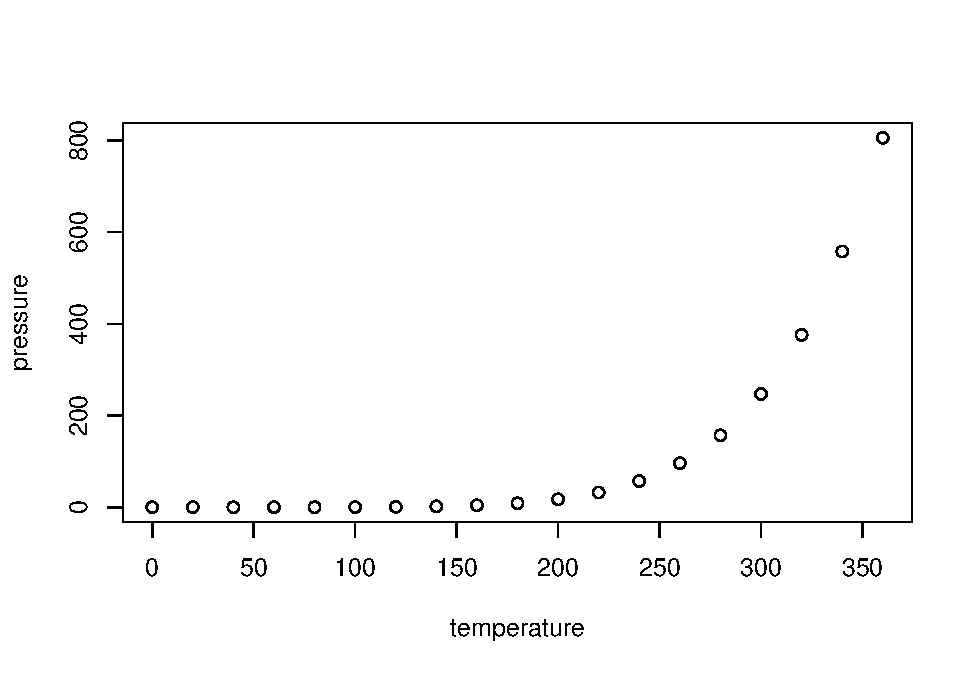
\includegraphics{trialanderror_files/figure-latex/pressure-1.pdf}

Note that the \texttt{echo\ =\ FALSE} parameter was added to the code
chunk to prevent printing of the R code that generated the plot.

\end{document}
